%!TEX root = ../report.tex

%
% Architecture
%

\section{Architecture} % (fold)
\label{sec:architecture}

This work will follow the architecture described in Figure~\ref{fig:architecture}.
There will be a module in Racket that will provide a Racket interface for the rest of the system using \emph{Racket FFI} and is through this that the users will mostely interact with the system. This will be a layer that will not have an impact on performance. 

\begin{figure}[htbp]
	\centering
	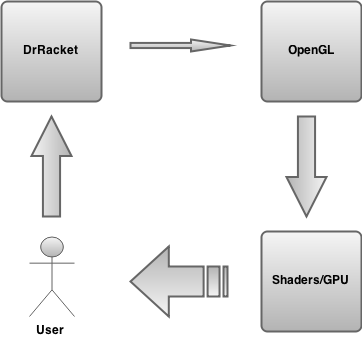
\includegraphics[width=0.95\textwidth]{img/Architecture/architecture1.png}
	\caption{High Level Architecture}
	\label{fig:architecture}
\end{figure}

The secont step is the OpenGL layer, that implement the Racket interface and than create the window and manage user input. The functions provided to Racket will create here the description of the geometry that will be \emph{amplified} in the next phase. This description is one $GL\_POINT$ per geometric primitive that represent the position of that primitive and it is also embebed with an array of floats that encode the type of geometry and specific information like size or number of sides.

In the last step are the shaders, where most of the work is done. This recives the small description of the geometry and gerates the primitives to be drawn. To achieve this, it is applied the concept of geometry amplification. The 

This architecture significantly reduces the amount of data that is moved between layers and takes advantage of the power that recent GPUs have.

For intance the folowing code results in the Figure~\ref{fig:pic1} that is a procedural generated model of a city with ~40k buildings.

%explicar exemplo

\begin{lstlisting}[frame=single,language=Lisp]  % Start your code-block

(start 0)
(city 100)
(init)
\end{lstlisting}

\begin{figure}[htb]
	\centering
	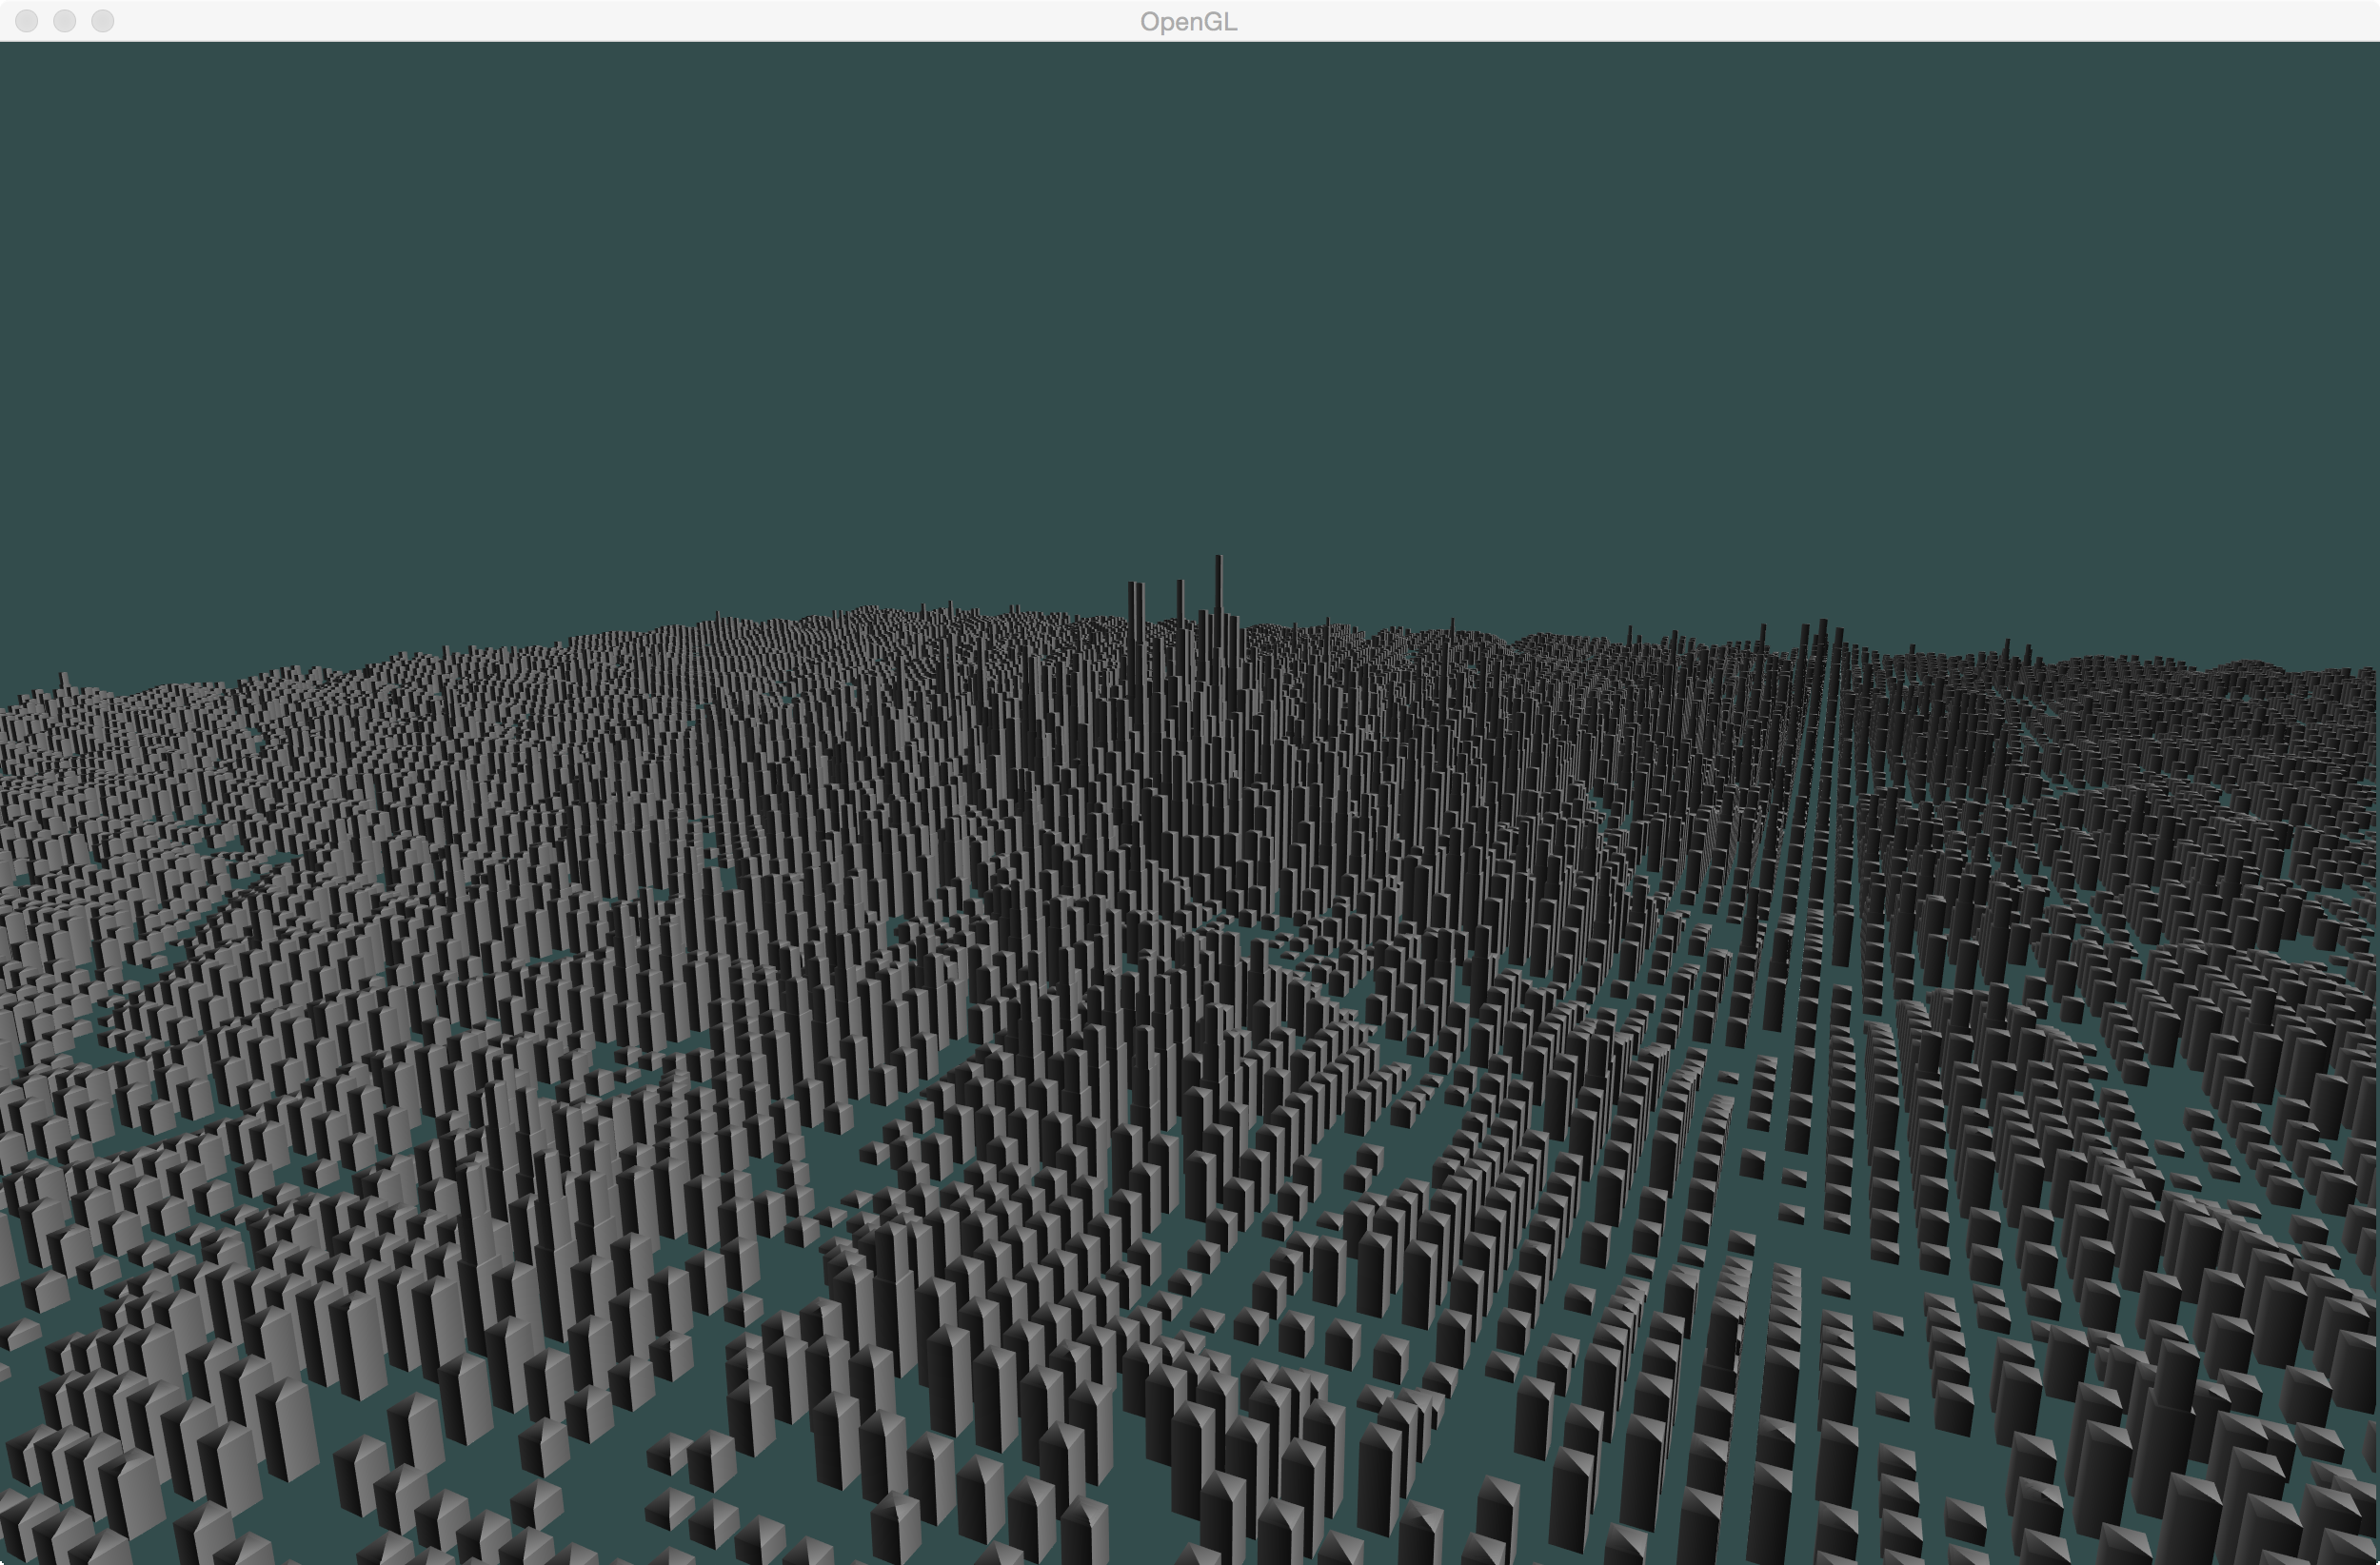
\includegraphics[width=0.95\textwidth]{img/Solution/City2-100*100.png}
	\caption{City Example}
	\label{fig:pic1}
\end{figure}



% section architecture (end)
